\documentclass[10pt]{beamer}

\usetheme{metropolis}
\usepackage{appendixnumberbeamer}

\usepackage[T1]{fontenc} % Use 8-bit encoding that has 256 glyphs
\usepackage[utf8]{inputenc}

\usepackage[english,italian]{babel}

\usepackage{booktabs}
\usepackage[scale=2]{ccicons}

\usepackage{pgfplots}
\usepgfplotslibrary{dateplot}

\usepackage{xspace}
\newcommand{\themename}{\textbf{\textsc{metropolis}}\xspace}

\title{GRAZIE. LUCI E RABBIA. SPAZIO.}
\subtitle{\emph{charms, thanks, graces, Charites\ldots Lights and Rage. Space.} \\ \vfill International ilSUONO Contemporary Music Academy}
\date{\today}

\author{Giuseppe Silvi}
\institute{\color{mDarkBrown}{\textbf{Città di Castello}}}
%\titlegraphic{\hfill\includegraphics[height=1.5cm]{Conservatorio-purple.png}}

\definecolor{mDarkBrown}{RGB}{74, 130, 113}%{HTML}{604c38}
\definecolor{mDarkTeal}{RGB}{81,69,148}%{HTML}{23373b}
\definecolor{mLightBrown}{RGB}{74, 130, 113}%{HTML}{EB811B}
\definecolor{mLightGreen}{RGB}{74, 130, 113}

\begin{document}

\maketitle

%--------------------------------------------------------------------------
%- INDEX ------------------------------------------------------------------
%--------------------------------------------------------------------------

%{%
%\setbeamertemplate{frame footer}{\color{mDarkBrown}{\textbf{GIUSEPPE SILVI. GLRS. 2018}}}
%\begin{frame}[fragile]{INDEX}
%  \setbeamertemplate{section in toc}[sections numbered]
%  \tableofcontents[
%      %hideallsubsections
%      ]
%\end{frame}
%}

%--------------------------------------------------------------------------
%- SECTION ----------------------------------------------------------------
%--------------------------------------------------------------------------

\section{WHO AM I} 

{%
\setbeamertemplate{frame footer}{\color{mDarkBrown}{\textbf{International ilSUONO Contemporary Music Academy 2018}}}

\begin{frame}[fragile]{\textbf{LIKE, DON'T LIKE}}

I like acoustical instruments.

I Like loudspeaker and electro-acoustical stuff.

I don't like the equilibrium between acoustical instruments and traditional loudspeakers.

Most time (in the music of others) I don't like the perceptual balance between acoustics and electro-acoustics.

I'm not interested in discography and recording technique that "popularize" the sound (magnification and un-naturalizing of sound).

\end{frame}
}

%--------------------------------------------------------------------------

{%
\setbeamertemplate{frame footer}{\color{mDarkBrown}{\textbf{International ilSUONO Contemporary Music Academy 2018}}}

\begin{frame}[fragile]{\textbf{OBSESSION}}

The emotional and physical perception of the vibrating matter.

\end{frame}
}

%--------------------------------------------------------------------------
%- SECTION ----------------------------------------------------------------
%--------------------------------------------------------------------------

{%
\setbeamertemplate{frame footer}{\color{mDarkBrown}{\textbf{International ilSUONO Contemporary Music Academy 2018}}}

\begin{frame}[fragile]{\textbf{riPercussioni}}

for Percussion and Space

\bigskip

\emph{“Noi musicisti siamo sempre stati schiavi del tempo”} \\
(We musicians have always been slaves of time) \\- Mario Bertoncini, private discussion during rehearsal - 2012

\bigskip

\emph{“Il tempo, ieri come oggi, è sempre la, è come l'aria, e la musica vi è totalmente immersa. Ma questo suo tempo la musica lo usa, lo prevede e ce lo descrive in maniera sempre indiretta, parlando d'altro.”} \\
(Time, yesterday as today, is always there, it's like air, and music totally dips in it. But music uses its own time, it foresees it and describes it in an always indirect way, talking about something else.) \\- Luciano Berio, \emph{Che tempo che fa} - 1985
\end{frame}
}

%--------------------------------------------------------------------------
%- SECTION ----------------------------------------------------------------
%--------------------------------------------------------------------------

{%
\setbeamertemplate{frame footer}{\color{mDarkBrown}{\textbf{International ilSUONO Contemporary Music Academy 2018}}}

\begin{frame}[fragile]{\textbf{S.T.ONE}}

\textbf{S.T.ONE} {\it (Spherical Tetrahedral ONE)}

is a tetrahedral loudspeaker able to reproduce spherical sound field.

The S.T.ONE loudspeaker defines the simplest way to electro-acoustically describe a spherical sound shape.

\end{frame}
}

%--------------------------------------------------------------------------

\begin{frame}{S.T.ONE}
  \begin{figure}[htbp]
	\begin{center}
		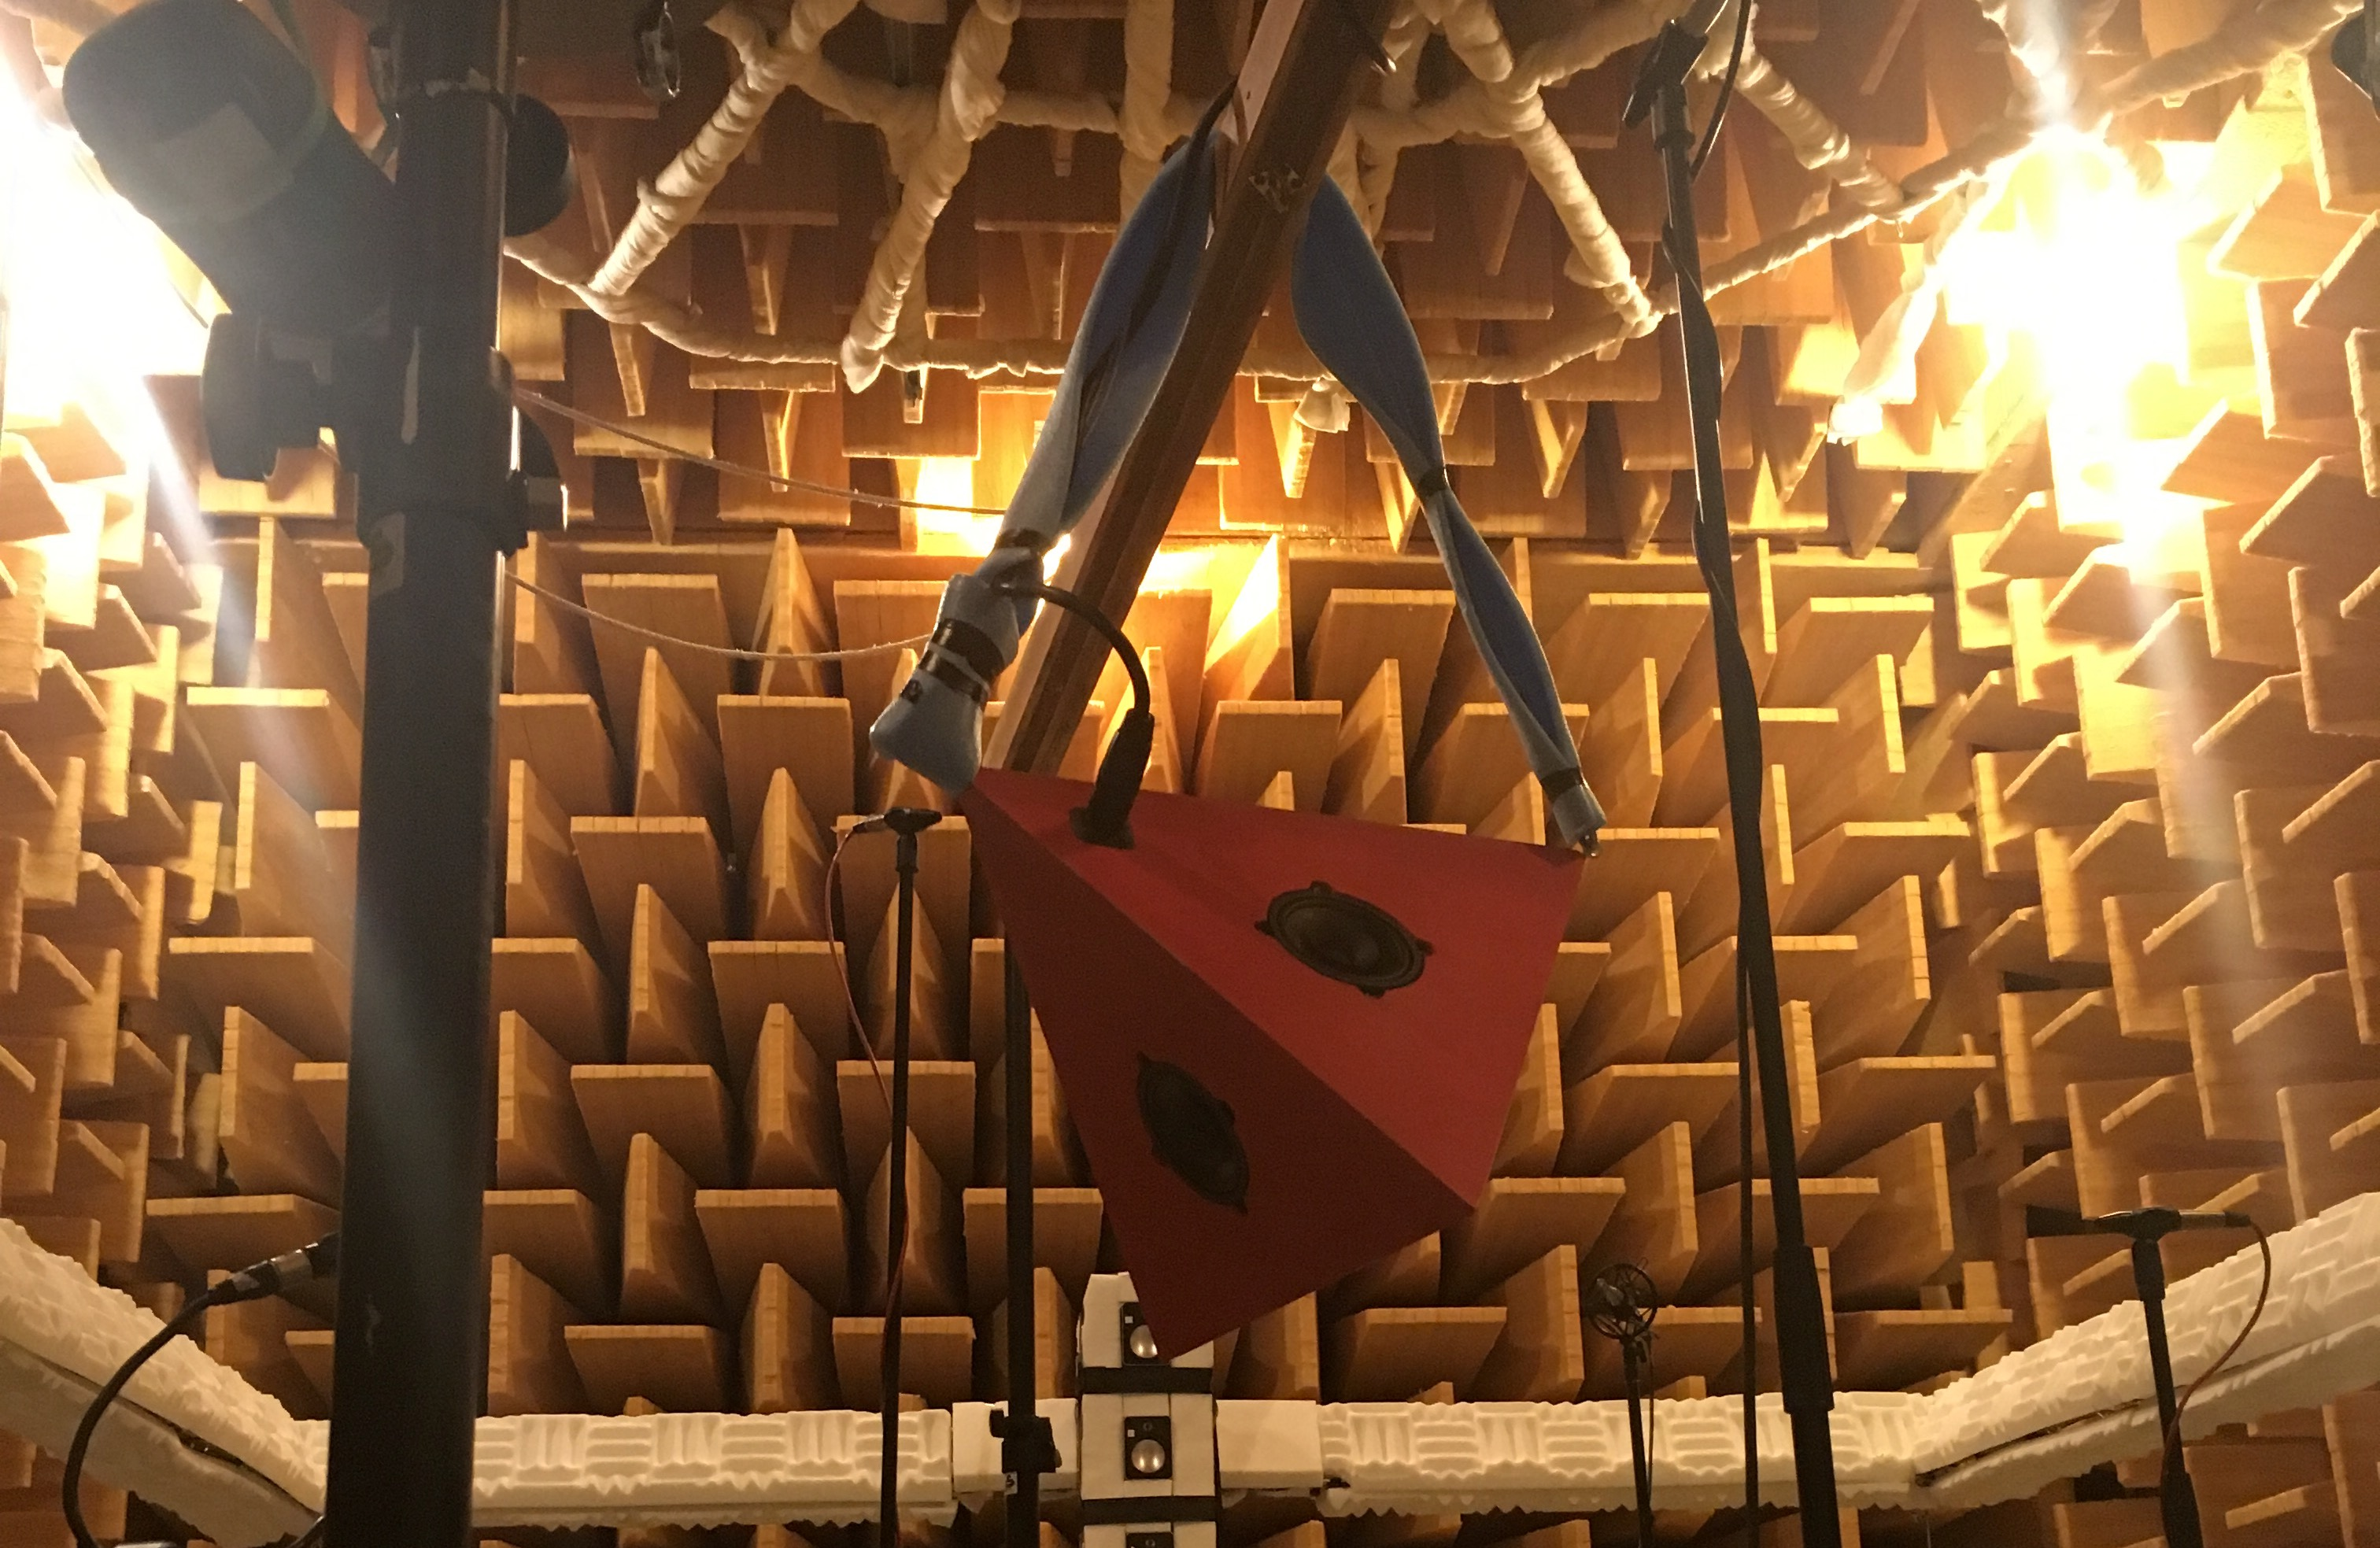
\includegraphics[width=1.\linewidth]{img/IMG_0612.JPG}
	\end{center}
	\end{figure}
\end{frame}

%--------------------------------------------------------------------------

\begin{frame}{S.T.ON3.L}
  \begin{figure}[htbp]
	\begin{center}
		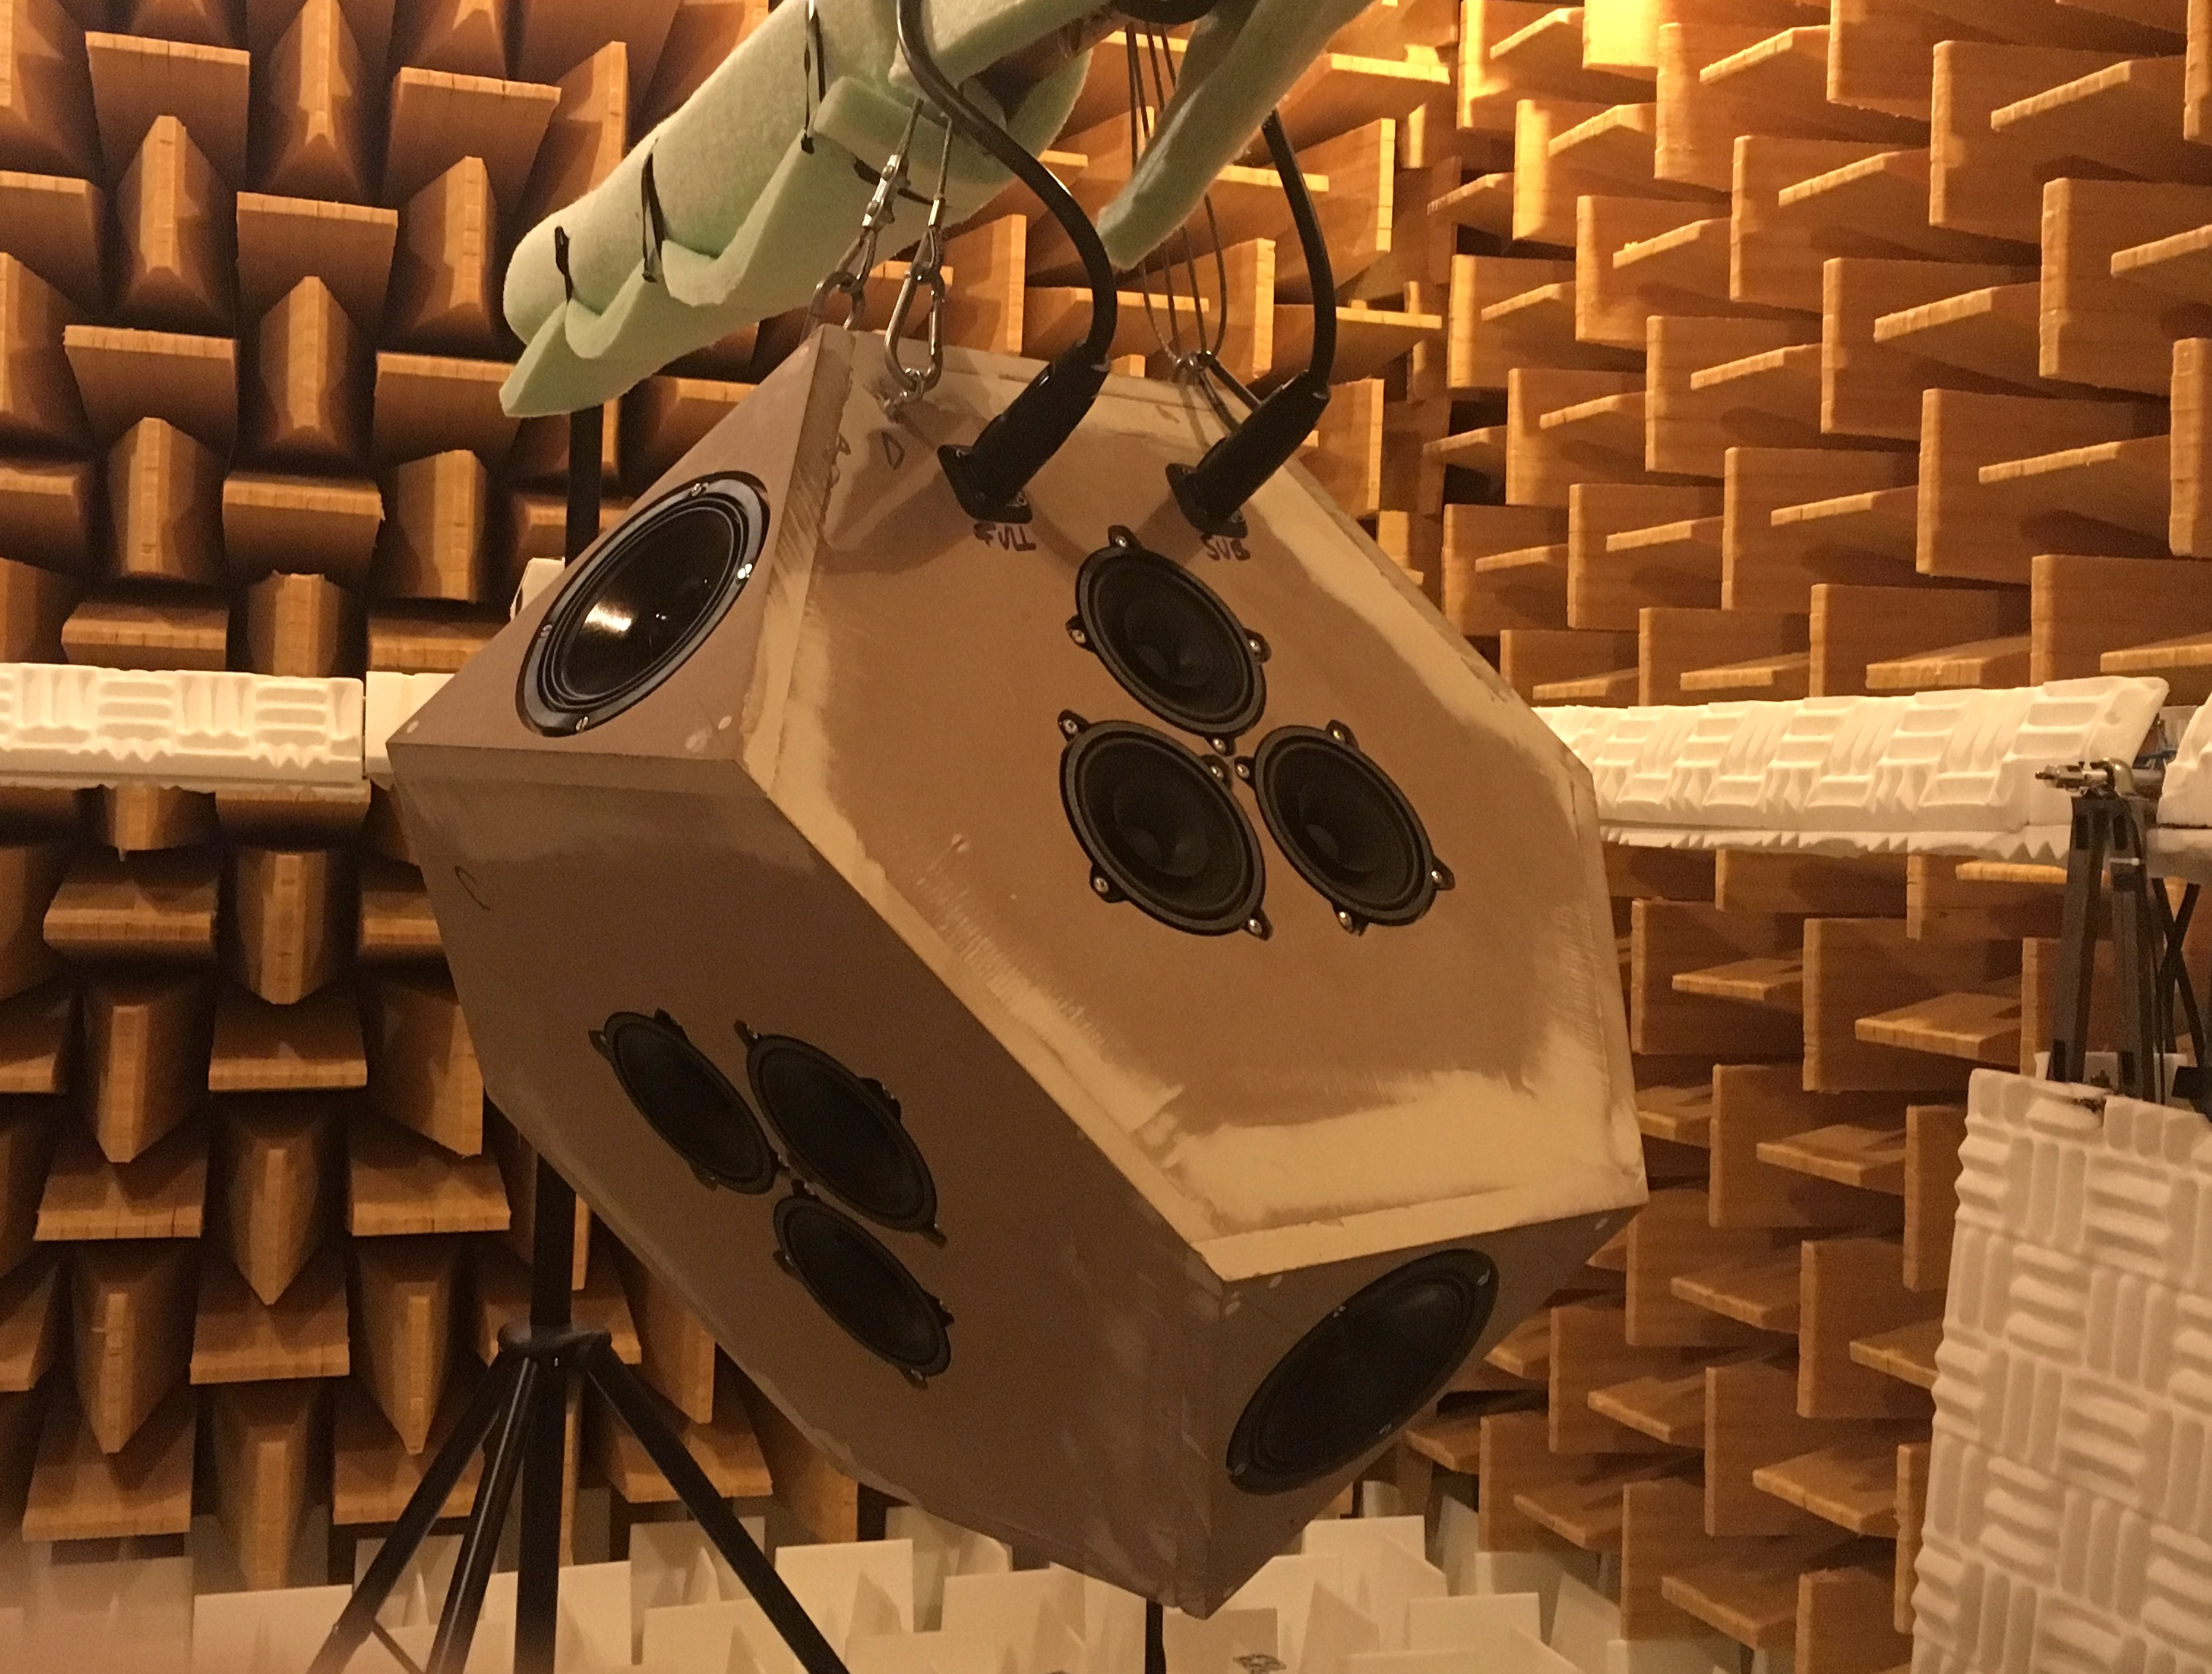
\includegraphics[width=1\linewidth]{img/IMG_0681.JPG}
	\end{center}
	\end{figure}
\end{frame}


%--------------------------------------------------------------------------

{%
\setbeamertemplate{frame footer}{\color{mDarkBrown}{\textbf{International ilSUONO Contemporary Music Academy 2018}}}
\begin{frame}[fragile]{\textbf{GRAZIE. LUCI E RABBIA. SPAZIO.}}

\emph{non quello architettonico. Acustico. Tangibile, della materia in vibrazione. Di ogni essenza sonora. Forma. Dove ogni parametro è carattere, cessa la sua indipendenza. Suono. Esiste solo nella sua completa complessità. Ognuno è esterno. Ognuno è vissuto, oppure immaginazione. La scoperta è tutto quello che ho, riempie e svuota d'emozione, nel tempo inaspettato di una vita.}

not the architectural one. Acoustical. Sensible, of the vibrating matter. Of any sound essence. Shape. Where every parameter is a character, its independence ceases. Sound. It exists only in its complete complexity. Each is external. Each is lived or imagination. It fills and empties with emotion, in the unexpected time of a lifetime.

\end{frame}
}

%--------------------------------------------------------------------------
%- QUESTIONS --------------------------------------------------------------
%--------------------------------------------------------------------------

\begin{frame}[standout]
  Questions?
\end{frame}

%\begin{frame}{SMERM}
%  \begin{figure}[htbp]
%	\begin{center}
%	\includegraphics[width=.9\linewidth]{../../gs-diagramma-SMERM/gs-diagramma-SMERM.pdf}
%	\end{center}
%	\end{figure}
%\end{frame}

%\begin{frame}[fragile]{Metropolis}
%
%  The \themename theme is a Beamer theme with minimal visual noise
%  inspired by the \href{https://github.com/hsrmbeamertheme/hsrmbeamertheme}{\textsc{hsrm} Beamer
%  Theme} by Benjamin Weiss.
%
%  Enable the theme by loading
%
%  \begin{verbatim}    \documentclass{beamer}
%    \usetheme{metropolis}\end{verbatim}
%
%  Note, that you have to have Mozilla's \emph{Fira Sans} font and XeTeX
%  installed to enjoy this wonderful typography.
%\end{frame}
%\begin{frame}[fragile]{Sections}
%  Sections group slides of the same topic
%
%  \begin{verbatim}    \section{Elements}\end{verbatim}
%
%  for which \themename provides a nice progress indicator \ldots
%\end{frame}
%
%\section{Title formats}
%
%\begin{frame}{Metropolis title formats}
%	\themename supports 4 different title formats:
%	\begin{itemize}
%		\item Regular
%		\item \textsc{Small caps}
%		\item \textsc{all small caps}
%		\item ALL CAPS
%	\end{itemize}
%	They can either be set at once for every title type or individually.
%\end{frame}
%
%{
%    \metroset{titleformat frame=smallcaps}
%\begin{frame}{Small caps}
%	This frame uses the \texttt{smallcaps} title format.
%
%	\begin{alertblock}{Potential Problems}
%		Be aware that not every font supports small caps. If for example you typeset your presentation with pdfTeX and the Computer Modern Sans Serif font, every text in small caps will be typeset with the Computer Modern Serif font instead.
%	\end{alertblock}
%\end{frame}
%}
%
%{
%\metroset{titleformat frame=allsmallcaps}
%\begin{frame}{All small caps}
%	This frame uses the \texttt{allsmallcaps} title format.
%
%	\begin{alertblock}{Potential problems}
%		As this title format also uses small caps you face the same problems as with the \texttt{smallcaps} title format. Additionally this format can cause some other problems. Please refer to the documentation if you consider using it.
%
%		As a rule of thumb: just use it for plaintext-only titles.
%	\end{alertblock}
%\end{frame}
%}
%
%{
%\metroset{titleformat frame=allcaps}
%\begin{frame}{All caps}
%	This frame uses the \texttt{allcaps} title format.
%
%	\begin{alertblock}{Potential Problems}
%		This title format is not as problematic as the \texttt{allsmallcaps} format, but basically suffers from the same deficiencies. So please have a look at the documentation if you want to use it.
%	\end{alertblock}
%\end{frame}
%}
%
%\section{Elements}
%
%\begin{frame}[fragile]{Typography}
%      \begin{verbatim}The theme provides sensible defaults to
%\emph{emphasize} text, \alert{accent} parts
%or show \textbf{bold} results.\end{verbatim}
%
%  \begin{center}becomes\end{center}
%
%  The theme provides sensible defaults to \emph{emphasize} text,
%  \alert{accent} parts or show \textbf{bold} results.
%\end{frame}
%
%\begin{frame}{Font feature test}
%  \begin{itemize}
%    \item Regular
%    \item \textit{Italic}
%    \item \textsc{Small Caps}
%    \item \textbf{Bold}
%    \item \textbf{\textit{Bold Italic}}
%    \item \textbf{\textsc{Bold Small Caps}}
%    \item \texttt{Monospace}
%    \item \texttt{\textit{Monospace Italic}}
%    \item \texttt{\textbf{Monospace Bold}}
%    \item \texttt{\textbf{\textit{Monospace Bold Italic}}}
%  \end{itemize}
%\end{frame}
%
%\begin{frame}{Lists}
%  \begin{columns}[T,onlytextwidth]
%    \column{0.33\textwidth}
%      Items
%      \begin{itemize}
%        \item Milk \item Eggs \item Potatoes
%      \end{itemize}
%
%    \column{0.33\textwidth}
%      Enumerations
%      \begin{enumerate}
%        \item First, \item Second and \item Last.
%      \end{enumerate}
%
%    \column{0.33\textwidth}
%      Descriptions
%      \begin{description}
%        \item[PowerPoint] Meeh. \item[Beamer] Yeeeha.
%      \end{description}
%  \end{columns}
%\end{frame}
%\begin{frame}{Animation}
%  \begin{itemize}[<+- | alert@+>]
%    \item \alert<4>{This is\only<4>{ really} important}
%    \item Now this
%    \item And now this
%  \end{itemize}
%\end{frame}
%\begin{frame}{Figures}
%  \begin{figure}
%    \newcounter{density}
%    \setcounter{density}{20}
%    \begin{tikzpicture}
%      \def\couleur{alerted text.fg}
%      \path[coordinate] (0,0)  coordinate(A)
%                  ++( 90:5cm) coordinate(B)
%                  ++(0:5cm) coordinate(C)
%                  ++(-90:5cm) coordinate(D);
%      \draw[fill=\couleur!\thedensity] (A) -- (B) -- (C) --(D) -- cycle;
%      \foreach \x in {1,...,40}{%
%          \pgfmathsetcounter{density}{\thedensity+20}
%          \setcounter{density}{\thedensity}
%          \path[coordinate] coordinate(X) at (A){};
%          \path[coordinate] (A) -- (B) coordinate[pos=.10](A)
%                              -- (C) coordinate[pos=.10](B)
%                              -- (D) coordinate[pos=.10](C)
%                              -- (X) coordinate[pos=.10](D);
%          \draw[fill=\couleur!\thedensity] (A)--(B)--(C)-- (D) -- cycle;
%      }
%    \end{tikzpicture}
%    \caption{Rotated square from
%    \href{http://www.texample.net/tikz/examples/rotated-polygons/}{texample.net}.}
%  \end{figure}
%\end{frame}
%\begin{frame}{Tables}
%  \begin{table}
%    \caption{Largest cities in the world (source: Wikipedia)}
%    \begin{tabular}{@{} lr @{}}
%      \toprule
%      City & Population\\
%      \midrule
%      Mexico City & 20,116,842\\
%      Shanghai & 19,210,000\\
%      Peking & 15,796,450\\
%      Istanbul & 14,160,467\\
%      \bottomrule
%    \end{tabular}
%  \end{table}
%\end{frame}
%\begin{frame}{Blocks}
%  Three different block environments are pre-defined and may be styled with an
%  optional background color.
%
%  \begin{columns}[T,onlytextwidth]
%    \column{0.5\textwidth}
%      \begin{block}{Default}
%        Block content.
%      \end{block}
%
%      \begin{alertblock}{Alert}
%        Block content.
%      \end{alertblock}
%
%      \begin{exampleblock}{Example}
%        Block content.
%      \end{exampleblock}
%
%    \column{0.5\textwidth}
%
%      \metroset{block=fill}
%
%      \begin{block}{Default}
%        Block content.
%      \end{block}
%
%      \begin{alertblock}{Alert}
%        Block content.
%      \end{alertblock}
%
%      \begin{exampleblock}{Example}
%        Block content.
%      \end{exampleblock}
%
%  \end{columns}
%\end{frame}
%\begin{frame}{Math}
%  \begin{equation*}
%    e = \lim_{n\to \infty} \left(1 + \frac{1}{n}\right)^n
%  \end{equation*}
%\end{frame}
%\begin{frame}{Line plots}
%  \begin{figure}
%    \begin{tikzpicture}
%      \begin{axis}[
%        mlineplot,
%        width=0.9\textwidth,
%        height=6cm,
%      ]
%
%        \addplot {sin(deg(x))};
%        \addplot+[samples=100] {sin(deg(2*x))};
%
%      \end{axis}
%    \end{tikzpicture}
%  \end{figure}
%\end{frame}
%\begin{frame}{Bar charts}
%  \begin{figure}
%    \begin{tikzpicture}
%      \begin{axis}[
%        mbarplot,
%        xlabel={Foo},
%        ylabel={Bar},
%        width=0.9\textwidth,
%        height=6cm,
%      ]
%
%      \addplot plot coordinates {(1, 20) (2, 25) (3, 22.4) (4, 12.4)};
%      \addplot plot coordinates {(1, 18) (2, 24) (3, 23.5) (4, 13.2)};
%      \addplot plot coordinates {(1, 10) (2, 19) (3, 25) (4, 15.2)};
%
%      \legend{lorem, ipsum, dolor}
%
%      \end{axis}
%    \end{tikzpicture}
%  \end{figure}
%\end{frame}
%\begin{frame}{Quotes}
%  \begin{quote}
%    Veni, Vidi, Vici
%  \end{quote}
%\end{frame}
%
%{%
%\setbeamertemplate{frame footer}{My custom footer}
%\begin{frame}[fragile]{Frame footer}
%    \themename defines a custom beamer template to add a text to the footer. It can be set via
%    \begin{verbatim}\setbeamertemplate{frame footer}{My custom footer}\end{verbatim}
%\end{frame}
%}
%
%\begin{frame}{References}
%  Some references to showcase [allowframebreaks] \cite{knuth92,ConcreteMath,Simpson,Er01,greenwade93}
%\end{frame}
%
%\section{Conclusion}
%
%\begin{frame}{Summary}
%
%  Get the source of this theme and the demo presentation from
%
%  \begin{center}\url{github.com/matze/mtheme}\end{center}
%
%  The theme \emph{itself} is licensed under a
%  \href{http://creativecommons.org/licenses/by-sa/4.0/}{Creative Commons
%  Attribution-ShareAlike 4.0 International License}.
%
%  \begin{center}\ccbysa\end{center}
%
%\end{frame}
%
%\begin{frame}[standout]
%  Questions?
%\end{frame}
%
%\appendix
%
%\begin{frame}[fragile]{Backup slides}
%  Sometimes, it is useful to add slides at the end of your presentation to
%  refer to during audience questions.
%
%  The best way to do this is to include the \verb|appendixnumberbeamer|
%  package in your preamble and call \verb|\appendix| before your backup slides.
%
%  \themename will automatically turn off slide numbering and progress bars for
%  slides in the appendix.
%\end{frame}
%
%\begin{frame}[allowframebreaks]{References}
%
%  \bibliography{demo}
%  \bibliographystyle{abbrv}
%
%\end{frame}

\end{document}
